\setcounter{secnumdepth}{3}
\chapter{Requirements Engineering}
\label{sec:requirementsengineering}
Dieses Kapitel zeigt die speziellen Eigenschaften des Requirements Engineering im bereich der Webentwicklung.

Früh in der Entwicklung einer Software muss man die Rahmenbedingungen festlegen. Zuerst wird gezeigt, für welche Geräte und Browser man sich spezialisieren und generalisieren kann. 

Danach werden die wichtigsten nicht funktionalen Eigenschaften einer Webseite aufgezeigt und zum Schluss noch weitere wichtige Aspekte des Requirement Engineerings.

\section{Endgeräte}
Es gibt verschiedene Endgeräte, welche die Webseite darstellen müssen. 
\begin{itemize}
\item PC
\item Mobile
\item Tablet
\item E-Reader
\item Spielkonsolen
\end{itemize}

Als erster Punkt des Requirements Engineering sind die Geräte aufgeführt, da davon vieles abhängt. Zum Beispiel die Grösse des Bildschirmes, die Grösse des Eingabegerätes (Maus, Finger), die Bandbreite und noch weitere Punkte.

Für die verschiedenen Bildschirmgrössen gibt es zwei verschiedene Ansätze, die im Unterkapitel \ref{sec:requirementsengineerin:endgeraete:responsivevsadaptive} \nameref{sec:requirementsengineerin:endgeraete:responsivevsadaptive} beschrieben werden.

Dem Problem der Bandbreite nimmt sich das Kapitel \ref{sec:requirementsengineerin:endgeraete:bandbreite} \nameref{sec:requirementsengineerin:endgeraete:bandbreite} an.

\subsection{Responsive- vs Adaptive Web Design}
\label{sec:requirementsengineerin:endgeraete:responsivevsadaptive}
\footcite{Responsive_vs_Adaptive_Design_2015-05-31}
Beim \gls{rwdLabel} wird eine Seite generiert, die sich der Bildschirmgrösse anpasst, wo hingegen beim \gls{awdLabel} für verschiedene Bilschirmgrössen jeweils ein anderes Layout ausgeliefert wird.

\begin{figure}[H]
  \centering
  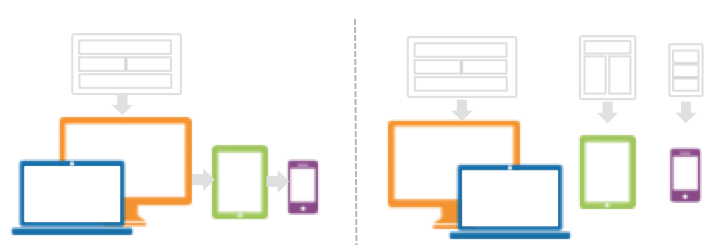
\includegraphics[width=0.9\textwidth]{images/rwd-vs-awd.png}
  \caption{Responsive- vs Adaptive Web Design\footcite{Responsive_vs_Adaptive_Design_for_UI_2015-05-31}}
  \label{fig:requirementsengineerin:endgeraete:responsivevsadaptive:comparision}
\end{figure}

Eim \gls{rwdLabel} liefert der Server für jedes Endgerät das selbe \Gls{glos:htmlLabel} aus. Die Elemente ordnen sich jedoch auf den verschiedenen Bildschirmgrössen anders an. Die folgende Grafik illustriert dieses vorgehen.

\begin{figure}[H]
  \centering
  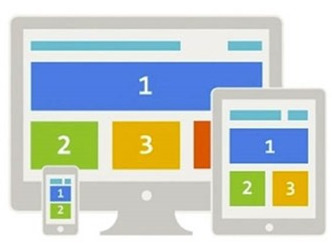
\includegraphics[width=0.4\textwidth]{images/rwd.jpg}
  \caption{Responsive Web Design\footcite{The_Difference_Between_Adaptive_Design_And_Responsive_Design_2015-05-31}}
  \label{fig:requirementsengineerin:endgeraete:responsivevsadaptive:rwd}
\end{figure}

Der Vorteil an dieser Variante ist es, dass keine Überprüfung der Bildschirmgrösse nötig ist und auf dem Bildschirm immer eine angepasste Ansicht ermöglicht wird. Auch wenn man die grösse des Browserfensters anpasst erhällt man immer eine passende Ansicht. Die Programmierung wird dadurch vereinfacht, dass nur eine \Gls{glos:htmlLabel} Seite generiert werden muss. Jedoch wird das Layout komplizierter und es müssen mehr Daten an das Engerät ausgeliefert werden.

Beim \gls{awdLabel} werden eigene \Gls{glos:htmlLabel} Seiten für die verschiedenen Auflösungen gepflegt. Um den selben Umfang wie das \gls{rwdLabel} zu ermöglichen, müssen die folgenden sechs Bildschirmbreiten gepflegt werden:
\begin{itemize}
\item 320px
\item 480px
\item 760px
\item 960px
\item 1200px
\item 1600px
\end{itemize}

Generell macht es Sinn ein \gls{rwdLabel} zu pflegen, da der Pflegeaufwand generell geringer ausfällt. Es gibt jedoch auch Gründe für ein \gls{awdLabel}. Zum Beispiel wenn eine bestehende Seite für mobile Geräte angepasst werden muss ist der Aufwand oft geringer, wenn man eine separate Ansicht dafür umsetzt. Die Ladezeiten für ein \gls{awdLabel} sind meistens auch besser, was folgende Tabelle aufzeigt. 
Für diesen Test\footcite{Adaptive_vs_Responsive_Web_Design_Which_Is_Right_for_Your_Site_-_Catchpoints_Blog_2015-06-01} wurden 15 Webseiten aus den \textit{Alexa Top 100 ranking (US)} Pages ausgesucht und analysiert.

\begin{center}
    \begin{tabular}{ | l | l | l |}
    \hline
    Metrik & \gls{awdLabel} & \gls{rwdLabel} \\ \hline
    Antwortzeit & 568 ms & 1'202 ms \\ \hline
    Zeit bis das Dokument vollständig geladen ist & 1'536ms & 4'086 ms \\ \hline
	Bytes Downloaded & 2'474'326 kB & 4'229'363 kB \\ \hline
	Objekte Downloaded & 20 & 61 \\ \hline
    \end{tabular}
\end{center}

Die \gls{awdLabel} Webseiten sind in allen Bereichen schneller. Es kann abschliessend gesagt werden, dass \gls{awdLabel} zu bevorzugen ist, wenn es auf die Geschwindigkeit ankommt. Dies war früher der Fall für mobile Endgeräte, fällt jedoch mit den neuen schnelleren Internetgeschwindigkeiten weniger ins Gewicht. Es sollte demnach wenn möglich \gls{rwdLabel} eingesetzt werden, ausser wenn die Migration einer bestehenden Webseite zu viel Aufwand bedeutet.


\subsection{Bandbreite}
\label{sec:requirementsengineerin:endgeraete:bandbreite}
Vor nicht all zu langer Zeit war die Bandbreite für Desktop PC's noch begrenzt und es musste sehr auf die Grösse von Bildern und Multimedia Inhalten geachtet werden. Doch das Internet entwickelte sich rasch weiter. Heute ist es möglich mehrere Full-HD (1980x1200 Pixel) Videos gleichzeitig anzusehen. Auf mobilen Endgeräten sieht es jedoch anders aus. Das \gls{wapLabel} wurde 1997 eingeführt. Auf grosse Grafiken musste man da noch verzichten da das Laden zu lange dauerte. Darauf folgte \gls{gprsLabel}, \gls{edgeLabel}, G3 und schlussendlich \gls{hsdpaLabel}. Mit den letzten beiden sind Webseiten und Bilder kein Problem mehr, und mit \gls{hsdpaLabel} können auch Multimedia Inhalte komfortable unterwegs angesehen werden. Die Abdeckung ist jedoch noch nicht flächendeckend. Vor allem in ländlichen Gebieten wird oft noch auf die älteren Verfahren zurückgegriffen. Deshalb muss für mobile Geräte die Bandbreite immer noch berücksichtigt werden.

Um die Bandbreite zu schonen werden Caches in den Browsern eingesetzt. Grosse Bilder, die auf mehreren Seiten vorkommen, zum Beispiel Banner, werden damit nur einmal heruntergeladen und auf dem Endgerät gespeichert. Dadurch ist nur der erste Seitenaufruf langsam. Die darauf folgenden Ladezeiten lassen sich jedoch beträchtlich vermindern.